%\documentstyle[epsf,twocolumn]{jarticle}       %LaTeX2e仕様
\documentclass[twocolumn]{jarticle}     %pLaTeX2e仕様(platex.exeの場合)
% \documentclass[onecolumn]{ujarticle}   %pLaTeX2e仕様(uplatex.exeの場合)
%%%%%%%%%%%%%%%%%%%%%%%%%%%%%%%%%%%%%%%%%%%%%%%%%%%%%%%%%%%%%%
%%
%%  基本バージョン
%%
%%%%%%%%%%%%%%%%%%%%%%%%%%%%%%%%%%%%%%%%%%%%%%%%%%%%%%%%%%%%%%%%
\setlength{\topmargin}{-45pt}
%\setlength{\oddsidemargin}{0cm}
\setlength{\oddsidemargin}{-7.5mm}
%\setlength{\evensidemargin}{0cm}
\setlength{\textheight}{24.1cm}
%setlength{\textheight}{25cm}
\setlength{\textwidth}{17.4cm}
%\setlength{\textwidth}{172mm}
\setlength{\columnsep}{11mm}

%\kanjiskip=.07zw plus.5pt minus.5pt


% 【節が変わるごとに (1.1)(1.2) … (2.1)(2.2) と数式番号をつけるとき】
%\makeatletter
%\renewcommand{\theequation}{%
%\thesection.\arabic{equation}} %\@addtoreset{equation}{section}
%\makeatother

%\renewcommand{\arraystretch}{0.95} 行間の設定
%%%%%%%%%%%%%%%%%%%%%%%%%%%%%%%%%%%%%%%%%%%%%%%%%%%%%%%%
%\usepackage{graphicx}   %pLaTeX2e仕様(\documentstyle ->\documentclass)
\usepackage[dvipdfmx]{graphicx}
\usepackage{subcaption}
\usepackage{multirow}
\usepackage{amsmath}
\usepackage{url}
\usepackage{ulem}
\usepackage{algorithm}
\usepackage{algorithmic}
\usepackage{listings} %,jlisting} %日本語のコメントアウトをする場合jlistingが必要
%ここからソースコードの表示に関する設定
\lstset{
  basicstyle={\ttfamily},
  identifierstyle={\small},
  commentstyle={\smallitshape},
  keywordstyle={\small\bfseries},
  ndkeywordstyle={\small},
  stringstyle={\small\ttfamily},
  frame={tb},
  breaklines=true,
  columns=[l]{fullflexible},
  numbers=left,
  xrightmargin=0zw,
  xleftmargin=3zw,
  numberstyle={\scriptsize},
  stepnumber=1,
  numbersep=1zw,
  lineskip=-0.5ex
}
%%%%%%%%%%%%%%%%%%%%%%%%%%%%%%%%%%%%%%%%%%%%%%%%%%%%%%%%
\begin{document}

	%bibtex用の設定
	%\bibliographystyle{ujarticle}

	\twocolumn[
		\noindent
		\hspace{1em}
		2020 年 5 月 15 日
		ゼミ資料
		\hfill
		B4 杉山 竜弥
		\vspace{2mm}

		\hrule
		\begin{center}
			{\Large \bf 進捗報告}
		\end{center}
		\hrule
		\vspace{9mm}
	]

	% ‚ここから 文章 Start!
\section{今週やったこと}
\begin{itemize}
	\item {入れ替えコードの実装と実験少し}
\end{itemize}

\section{問題設定}
% 何を入力として何を出力とするかを明確に定義

 データを正解と不正解に分割して学習する以下のアルゴリズム1を考える.

	\begin{algorithm}
		\caption{Swap two datasets}
		\label{alg1}
		\begin{enumerate}{ % itemize, enumerate, description
			\item{データ 2N 抜き出す}
			\item{そのデータを ランダムに N(A) と N(B)に分ける.}
			\item{X : A → train, B → test で学習}
			\item{Y : B → train, A → test で学習}
			\item{3.と4.で test でミスしたデータを調べる}
			\item{A をテストとしたとき失敗したデータと B をテストとしたとき成功したデータを入れ替える.ただし, 同じクラスのデータ同士.}
			\item{モデルを初期化して, 3.に戻る.}
		}\end{enumerate}
			% \begin{algorithmic}
			% \end{algorithmic}
	\end{algorithm}

	前回とは異なり, データのクラスが同じもの同士を入れ替えることで, データセットのクラス比が変化しないようにした.
  学習中に入れ替えるのではなく, 学習が終わった後入れ替え, 再び学習する際にモデルのパラメータは初期化した.


\section{実験}

	\begin{table}[tb]
		\begin{center}
			\caption{実験の設定}
			\begin{tabular}{|c|c|} \hline
				dataset & cifar10 \\
				data N & 5,000 / model \\ \hline
				task & 10クラス識別 \\
				input & image(3x32x32) \\
				output & class(10) \\ \hline
				model & CNN(16層) \\
				optim & SDG (lr=0.001, moment=0.9) \\
				loss & Cross Entropy Loss \\ \hline
				batch size & 16 \\
				epoch & 30 \\ \hline
        swap & 10 \\ \hline
			\end{tabular}
			\label{tab:setting}
		\end{center}
	\end{table}

実験設定は表\ref{tab:setting}とした. 30 epoch学習した後, データを入れ替える手順を10 回行った. はじめは50 epochに設定したが, 長時間の実験をするとGoogle Colabがいつの間にか中断したため, 30 epochと短めにした.

\subsection{結果}

テストの精度は図\ref{fig:accuracy}に示した. 横軸はデータを入れ替えた回数で, 今回は10 回である. 1回目の精度が40 ~ 45 [\%]でこれは入れ替えなかった場合の指標である. 学習epoch数が少なかったために精度が高まらない結果となった. その後入れ替えを行うたびに精度は減少し, 共に20 \%程度となった. 条件が異なるので単純に比較できないが, 前回まで手順3が手順4より大幅に低い精度であったため, 予想を裏切る結果であった.
入れ替えをランダムに行った場合は精度がほとんど変わっていないため, 入れ替え操作が精度に影響していると言える.


\begin{figure}[tb]
	\begin{center}
		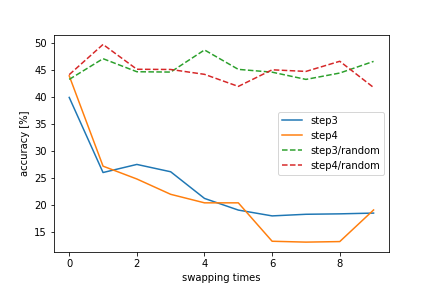
\includegraphics[clip,width=8.5cm]{accuracy.png}
		\caption{学習後モデルのテストの精度 
		実線がテスト結果で入れ替えた場合,
    点線がランダムに入れ替えた場合}
		\label{fig:accuracy}
	\end{center}
\end{figure}

図\ref{fig:accuracy_start}に学習がまだ進んでいない初期の0~epoch目のテストの結果を示した. ベースラインは10 \%であるため, 交換が重ねられるごとにデータセットの難しさが高まっていると思われる. また手順3と手順4を比較すると, 不正解データが集められた手順4がより難しいことが分かる.

\begin{figure}[tb]
	\begin{center}
		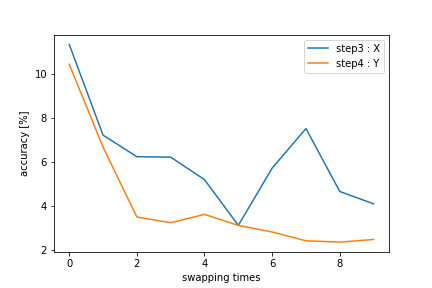
\includegraphics[clip,width=8.5cm]{accuracy_start.png}
		\caption{0epoch目のテストの精度 (ベースライン:10 \%) 
		実線の青が手順3, 橙が手順4}
		\label{fig:accuracy_start}
	\end{center}
\end{figure}

入れ替えられたデータの数は, 図\ref{fig:class}のようにラベルのクラスを区別して示した. データサンプル数は5000なので, 1回目の入れ替えでは2000個の半数近くが交換されていた. その後も1000個程度が常に入れ替えられている. クラスの比率はあまり偏りが見られず, ほぼ同数であった.

\begin{figure*}[tb]
  \begin{center}
    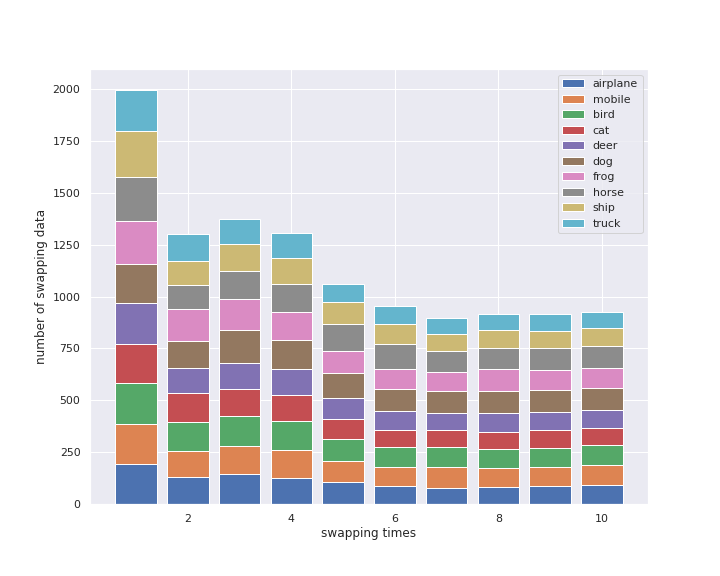
\includegraphics[clip,width=16.5cm]{swapclass.png}
    \caption{入れ替えたデータのクラスラベル}
    \label{fig:class}
  \end{center}
\end{figure*}

\section{考察}
% 精度が出ない,とかだけではなく自分なりの考察を示す
図\ref{fig:accuracy}の精度は両方とも減少した. 訓練セットとテストセットの偏りが大きくなるにつれて, 学習してないテスト画像を間違えたと思われる. パラメータは初期化しているため, モデルが学習した画像にテストセットは含まれていない. 従って精度が増加する要因はないと考えられる.

データの入れ替え数ではラベル比に偏りが見られなかったため, 交換されるデータの中で交換頻度の高い画像などを見たい.

パラメータのチューニングに時間がかかったので, optunaが適用できるかを調べたい.

\section{今後の予定}
% なんとなくなんかの勉強をするとかではなく具体的に
\begin{itemize}
	\item {入れ替え頻度の高いデータの分析}
\end{itemize}

\section{ソースコード}
% 埋め込みでもGitでもいいので参照できるように

% \begin{lstlisting}[caption=cnn,label=model_cnn]
% code
% \end{lstlisting}


% 参考文献リスト
\bibliographystyle{unsrt}
\bibliography{ref}
\end{document}
